\documentclass[14pt,a4paper,oneside]{extbook}
\usepackage[utf8]{vietnam}
\usepackage{amsmath,amssymb,mathrsfs,fancyhdr,enumerate,multirow,makecell}
\usepackage{tkz-euclide,tikz-3dplot,tikz,tkz-tab}
\usetikzlibrary{arrows.meta,calc,intersections,angles,quotes,backgrounds,shapes.geometric,patterns,through,shadows,positioning}
\usepackage{yhmath}
\usepackage[top=0.7cm, bottom=0.7cm, left=1.0cm, right=1.0cm, headheight=16pt, headsep=3mm, footskip=5mm]{geometry}
\usepackage[hidelinks,unicode]{hyperref}
\usepackage{qrcode}
\usepackage[many]{tcolorbox}
\usepackage{fontawesome}

\pagestyle{fancy}
\fancyhf{}
\fancyhead[L]{\footnotesize\bfseries\color{teal!85!black}\faBook~SỔ TAY KIẾN THỨC TOÁN 5}
\fancyhead[R]{\footnotesize\bfseries\color{blue!85!black}Lớp Toán Thầy Lĩnh -- loptoanthaylinh.vn}
\fancyfoot[C]{\footnotesize\bfseries\color{gray!80!black}-- Sổ tay kiến thức: Bài 16. Các đơn vị đo diện tích --}
\renewcommand{\headrulewidth}{0.4pt}

\begin{document}

% --- BANNER TIÊU ĐỀ BÀI HỌC ---
\noindent
\begin{tcolorbox}[
  enhanced,
  colback=teal!8!white,
  colframe=teal!80!black,
  arc=3mm,
  boxrule=1.1pt,
  width=\linewidth,
  halign=center,
  top=2.2mm, bottom=2.2mm,
  left=3mm, right=3mm,
  drop fuzzy shadow
]
  {\large\bfseries\color{teal!95!black}\faBookmark\ BÀI 16. CÁC ĐƠN VỊ ĐO DIỆN TÍCH}\\[2pt]
  {\scriptsize\color{black!75}\itshape Bảng đầy đủ 7 đơn vị đo diện tích từ km2 đến mm2 và quy tắc dịch chuyển chữ số trên 1 trang A4}
\end{tcolorbox}

\vspace{3.2mm}
% --- KHỐI 1: BẢNG TỔNG HỢP CẢ 7 ĐƠN VỊ ĐO DIỆN TÍCH ---
\noindent
\begin{tcolorbox}[
  enhanced,
  title={\footnotesize\bfseries\color{white}\faTable\ 1. Bảng đầy đủ các đơn vị đo diện tích},
  colback=blue!2!white,
  colframe=blue!75!black,
  arc=2.5mm, boxrule=0.8pt, top=1.8mm, bottom=1.8mm, left=2mm, right=2mm
]
  \scriptsize
  \centering
  \begin{tabular}{|c|c|c|c|c|c|c|}
    \hline
    \multicolumn{3}{|c|}{\textbf{Lớn hơn mét vuông}} & \textbf{Mét vuông} & \multicolumn{3}{c|}{\textbf{Bé hơn mét vuông}} \\ \hline
    $\text{km}^2$ & $\text{hm}^2$ ($\text{ha}$) & $\text{dam}^2$ & $\mathbf{m^2}$ & $\text{dm}^2$ & $\text{cm}^2$ & $\text{mm}^2$ \\ \hline
    $100\text{ hm}^2$ & $100\text{ dam}^2$ & $100\text{ m}^2$ & $\mathbf{1\ m^2}$ & $\frac{1}{100}\text{ m}^2$ & $\frac{1}{100}\text{ dm}^2$ & $\frac{1}{100}\text{ cm}^2$ \\ \hline
  \end{tabular}\\[3pt]
  {\tiny\color{blue!85!black}\bfseries Mỗi đơn vị diện tích gấp 100 lần đơn vị liền sau, và bằng $\frac{1}{100}$ đơn vị liền trước. Mỗi cột ứng với đúng 2 chữ số!}
\end{tcolorbox}

\vspace{3mm}

% --- KHỐI 2: NGUYÊN TẮC 2 CHỮ SỐ MỖI HÀNG ---
\noindent
\begin{minipage}[t]{0.52\textwidth}
  \begin{tcolorbox}[
    enhanced,
    title={\footnotesize\bfseries\color{white}\faKey\ 2. Nguyên tắc vàng ``2 chữ số mỗi cột''},
    colback=teal!2!white,
    colframe=teal!75!black,
    arc=2.5mm, boxrule=0.8pt, top=1.8mm, bottom=1.8mm, left=2.2mm, right=2.2mm
  ]
    \footnotesize
    Khi chuyển đổi đơn vị diện tích:\\
    $\bullet$ Đổi sang đơn vị liền sau (nhỏ hơn): Nhân với $100$ (hoặc dịch dấu phẩy sang phải \textbf{2 chữ số}).\\
    $\bullet$ Đổi sang đơn vị liền trước (lớn hơn): Chia cho $100$ (hoặc dịch dấu phẩy sang trái \textbf{2 chữ số}).\\
    \textit{VD:} $3,45\text{ m}^2 = 345\text{ dm}^2$.\\
    $7\text{ dm}^2 = 0,07\text{ m}^2$.
  \end{tcolorbox}
\end{minipage}%
\hfill
\begin{minipage}[t]{0.46\textwidth}
  \begin{tcolorbox}[
    enhanced,
    title={\footnotesize\bfseries\color{white}\faSearch\ 3. Phương pháp lập bảng nhẩm},
    colback=purple!2!white,
    colframe=purple!70!black,
    arc=2.5mm, boxrule=0.8pt, top=1.8mm, bottom=1.8mm, left=2mm, right=2mm
  ]
    \footnotesize
    Viết $4\text{ m}^2\ 5\text{ cm}^2$ ra $\text{m}^2$:\\
    \centering
    \begin{tabular}{|c|c|c|}
      \hline
      $\text{m}^2$ & $\text{dm}^2$ & $\text{cm}^2$ \\ \hline
      $4$ & $0\ 0$ & $0\ 5$ \\ \hline
    \end{tabular}\\[2pt]
    $\Rightarrow 4\text{ m}^2\ 5\text{ cm}^2 = 4,0005\text{ m}^2$.\\
    Không sợ thiếu bất kì chữ số $0$ nào!
  \end{tcolorbox}
\end{minipage}

\vspace{3mm}

% --- KHỐI 3: SƠ ĐỒ TƯ DUY ---
\noindent
\begin{tcolorbox}[
  enhanced,
  title={\footnotesize\bfseries\color{white}\faSitemap\ Sơ đồ tư duy: Bảng quy đổi diện tích},
  colback=yellow!2!white,
  colframe=teal!85!black,
  arc=3mm, boxrule=0.9pt, top=1.8mm, bottom=1.8mm, left=1.5mm, right=1.5mm,
  halign=center
]
  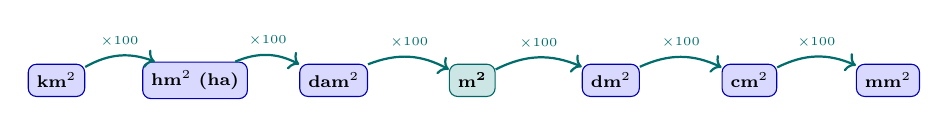
\begin{tikzpicture}[
    scale=0.88,
    every node/.style={transform shape},
    u/.style={rectangle, rounded corners=3pt, fill=blue!15, draw=blue!70!black, font=\bfseries\scriptsize, inner sep=3.5pt}
  ]
    \node[u] (u1) at (-6, 0) {$\text{km}^2$};
    \node[u] (u2) at (-4, 0) {$\text{hm}^2$ (ha)};
    \node[u] (u3) at (-2, 0) {$\text{dam}^2$};
    \node[u, fill=teal!20, draw=teal!80!black] (u4) at (0, 0) {$\mathbf{m^2}$};
    \node[u] (u5) at (2, 0) {$\text{dm}^2$};
    \node[u] (u6) at (4, 0) {$\text{cm}^2$};
    \node[u] (u7) at (6, 0) {$\text{mm}^2$};

    \foreach \i/\j in {u1/u2, u2/u3, u3/u4, u4/u5, u5/u6, u6/u7} {
      \draw[teal!85!black, thick, ->] (\i) to[bend left=25] node[above, font=\tiny] {$\times 100$} (\j);
    }
  \end{tikzpicture}
\end{tcolorbox}

\vspace{3mm}

% --- KHỐI 4: KỸ THUẬT NHẨM NHANH & BẪY TRẮC NGHIỆM ---
\noindent
\begin{minipage}[t]{0.54\textwidth}
  \begin{tcolorbox}[
    enhanced,
    title={\footnotesize\bfseries\color{white}\faBolt\ Cách bước qua nhiều đơn vị},
    colback=green!3!white,
    colframe=green!60!black,
    arc=2.5mm, boxrule=0.8pt, top=1.8mm, bottom=1.8mm, left=2.2mm, right=2.2mm
  ]
    \footnotesize
    Cứ qua $1$ bước đơn vị diện tích $\leftrightarrow$ dịch $2$ chữ số:\\
    $\bullet$ $\text{m}^2 \rightarrow \text{cm}^2$: Qua $2$ bước ($\text{dm}^2, \text{cm}^2$) $\rightarrow$ Dịch $4$ chữ số ($1\text{ m}^2 = 10\,000\text{ cm}^2$).\\
    $\bullet$ $\text{km}^2 \rightarrow \text{m}^2$: Qua $3$ bước $\rightarrow$ Dịch $6$ chữ số ($1\text{ km}^2 = 1\,000\,000\text{ m}^2$).
  \end{tcolorbox}
\end{minipage}%
\hfill
\begin{minipage}[t]{0.44\textwidth}
  \begin{tcolorbox}[
    enhanced,
    title={\footnotesize\bfseries\color{white}\faExclamationTriangle\ Mẹo tránh bẫy trắc nghiệm},
    colback=red!2!white,
    colframe=red!70!black,
    arc=2.5mm, boxrule=0.8pt, top=1.8mm, bottom=1.8mm, left=2.2mm, right=2.2mm
  ]
    \footnotesize
    $\bullet$ Rất nhiều học sinh nhầm giữa đơn vị đo \textbf{độ dài} (gấp kém $10$ lần) với đơn vị đo \textbf{diện tích} (gấp kém $100$ lần).\\
    $\bullet$ $1\text{ m} = 10\text{ dm}$ nhưng $1\text{ m}^2 = 100\text{ dm}^2$!
  \end{tcolorbox}
\end{minipage}

\end{document}
